%%% spell check: aug 29, 2014 
%%%% handouts:  pdfjam --landscape --nup '2x2' ecology3.pdf
%%%% handouts:  pdfjam --landscape ecology3.pdf

%\documentclass[handout]{beamer}
\documentclass[10pt]{beamer}
\usepackage{parskip}
\setlength{\parskip}{1.75ex}

\mode<presentation>
{\usetheme{Singapore}
\setbeamercovered{transparent}}

\title{R Minicourse Workshop, Part 3}

\author{\small Presented to the\\
        Washington State Deptment of Ecology\\
       September 2--3, 2014}

\date{\scriptsize Dr.~Robin Matthews, Institute for Watershed Studies\\
   Dr. Geoffrey Matthews, Computer Science Department\\
   Western Washington University}


\setbeamertemplate{blocks}[rounded][shadow=true]
\setbeamertemplate{footline}{\hspace*{5ex}Part 3 - Sept.~3, 2014 
   \hfill Page \insertframenumber \hspace{0.1ex} of
   \inserttotalframenumber \hspace*{5ex}
   \vspace*{2ex}}

\begin{document}
\lecture{R Minicourse}{Section 3}
\newcommand{\be}{\begin{enumerate}}
\newcommand{\ee}{\end{enumerate}}
\newcommand{\bi}{\begin{itemize}}
\newcommand{\ei}{\end{itemize}}
\newcommand{\bd}{\begin{description}}
\newcommand{\ed}{\end{description}}


\begin{frame}
\titlepage
\end{frame}

\begin{frame}
\frametitle{Bivariate Analysis Using {\color{red} \tt R}}
\framesubtitle{Correlation and Regression}

\bi
\item Regression measures the relationship between an independent
  variable ($x$) and one or more dependent variables ($y_{i}$)

\bi
\item Used to predict (model) unmeasured values of the dependent
  variable(s)
\ei

\item Correlation analysis measures the relationship between two
  variables that are not necessarily functionally dependent

\bi
\item Used to explore patterns in measured variables and to identify
  {\em indicators} that predict responses in other variables
\ei
\ei

\end{frame}

\begin{frame}
\frametitle{Correlation vs.~Regression}

{\small Correlation and regression examine {\em
    monotonic} relationships between variables}

\begin{center}
\resizebox{2.75in}{!}{
\includegraphics{./part3figures/regression1.ps}}
\end{center}
\end{frame}


\begin{frame}
\frametitle{Assumptions for Correlation and Regression}

\bi 
\item {\em Parametric} correlation ($r$) and simple linear regression
  ($r^2$) is based on several important assumptions: 

\bi
\item The samples were collected randomly 
\item The variables or linear residuals are normally distributed
\item The variance is constant (homoscedastic)
\item The relationship is monotonic ($\pm$linear)
\item The data do not contain outliers (or not very many)
\ei
\item {\em Nonparametric} correlation ($\rho$, $\tau$) does not
  require a linear relationship or homoscedasticity, but it still
  assumes that the relationship between x and y is monotonic
\ei
\end{frame}

\begin{frame}[fragile]
\frametitle{Correlation Analysis}
\bi
\item The strength of a correlation is measured using a
correlation coefficient (Pearson's $r$, Spearman's $\rho$, Kendall's $\tau$)

\hspace{5ex}$r = \frac{1}{n-1} \sum 
     \left( 
        \frac{x_{i}-{\overline x}}{s_{x}} \times 
        \frac{y_{i} - {\overline y}}{s_{y}} 
     \right)$

\hspace{5ex}$\rho$ is linear correlation computed on ranks

\hspace{5ex}$\tau = \frac{{\rm S}}{n(n-1)/2}$

{\scriptsize
\hspace{10ex}S = P - M\\
\hspace{10ex}P = number of times y increases with x;\\ 
\hspace{10ex}M = number of times y decreases as x increases\\
}

\item H$_{o}$: $r$ or $\rho$ or $\tau$ = 0 \hspace{0.5in} H$_{a}$: $r$ or $\rho$ or $\tau$  $\neq$ 0

\item $-1 \le r$ or $\rho$ or $\tau \le 1$
\ei
\end{frame}

\begin{frame}[fragile]
\frametitle{Correlation Analysis Using {\color{red} \tt R}}

Parametric and nonparametric correlation is done using {\color{red} \tt cor.test}

{\scriptsize
\color{red}

\verb%lakes <- read.csv("lakes.csv", T)%\\
\verb%attach(lakes)%\\
\verb%cor.test(alk, ph)%\\

\vspace{1ex}
\color{blue}
\verb%	Pearson's product-moment correlation%\\

\verb%data:  alk and ph %\\
\verb%t = 15.5074, df = 376, p-value < 2.2e-16%\\
\verb%alternative hypothesis: true correlation is not equal to 0 %\\
\verb%95 percent confidence interval:%\\
\verb% 0.5589116 0.6824434 %\\
\verb%sample estimates:%\\
\verb%      cor %\\
\verb%0.6245687 %\\

\color{red}
\vspace{2ex}
\verb%##### Nonparametric versions (all sig at p-value < 2.2e-16)%\\
\verb%cor.test(alk, ph, method="spearman")  #rho=0.6785801%\\
\verb%cor.test(alk, ph, method="kendall")   #tau=0.5030349%\\
}

\end{frame}




\begin{frame}[fragile]
\frametitle{Simple Linear Regression}

\bi
\item Simple linear regression is based on the  model: 

\hspace{5ex}$y_{i} = a + bx_{i} + \varepsilon_{i}$

\hspace{10ex}$a$ = intercept\\
\hspace{10ex}$b$ = slope\\
\hspace{10ex}$\varepsilon$ = residual for the i$^{th}$ observation

\item The strength of the regression is measured with the
  regression statistic or coefficient of determination ($r^2$)

\item H$_{o}$: $r^2$ = 0 \hspace{0.5in} H$_{a}$: $r^2\neq$ 0

\item $-1 \le r^2 \le 1$
\ei
\end{frame}

\begin{frame}[fragile]
\frametitle{Simple Linear Regressions Using {\color{red} \tt R}}

The easiest option for simple linear regressions is {\color{red} \tt lm}

{\scriptsize \color{red}
\verb%X <- c(1:10)%\\
\verb%Y <- c(49.8,51.6,53.7,53.9,55.1,56.5,57.4,57.9,58.9,60.8)%\\
\verb%##### Y is x+50, with "noise"%\\


\vspace{1ex}
\verb%lm(Y~X)%\\
\color{blue}
\verb%Call:%\\
\verb%lm(formula = Y ~ X)%\\

\verb%Coefficients:%\\
\verb%(Intercept)            X  %\\
\verb%     49.460        1.109  %\\

\vspace{2ex}
\verb%##### X = 1.109 * Y + 49.460%\\

\vspace{2ex}
\color{red}
\verb%##### Predicting Y for unmeasured values of X:%\\
\verb%predict(Yfit, list(X=6.7))%\\

\color{blue}
\verb%       1 %\\
\verb%56.89091 %\\

\vspace{2ex}
\color{red}
\verb%##### Predicting Y for all measured values of X:%\\
\verb%round(predict(Yfit),2)%\\
\color{blue}
\verb%    1     2     3     4     5     6     7     8     9    10 %\\
\verb%50.57 51.68 52.79 53.90 55.01 56.11 57.22 58.33 59.44 60.55 %\\
}

\end{frame}

\begin{frame}
\frametitle{Correlation/Regression}
\framesubtitle{Comparison Using Four Types of Curves}
\label{regression2}
\begin{center}
\resizebox{3in}{!}{
\includegraphics{./part3figures/regression2.ps}}
\end{center}
\end{frame}



\begin{frame}
\frametitle{Plotting Simple Linear Regressions Using {\color{red} \tt R}}
\begin{center}
\resizebox{3in}{!}{
\includegraphics{./part3figures/Y.ps}}
\end{center}
\end{frame}

\begin{frame}
\frametitle{Advanced Plotting Features - IWS Lakes Data}
\framesubtitle{Adding Confidence Intervals}
\begin{center}
\resizebox{3in}{!}{
\includegraphics{./part3figures/advanced1.ps}}
\end{center}

\end{frame}


\begin{frame}[fragile]
\frametitle{Syntax for Adding Confidence Intervals}

{\scriptsize
\color{red}
\verb%lakes = read.table("lakes.csv", T, sep=",")%\\
\verb%attach(lakes)%\\

\vspace{3ex}
\verb%### Step 1:  create linear model (chl ~ alk)%\\
\verb%alkchl.lm = lm(log10(chl) ~ alk)%\\

\vspace{3ex}
\verb%### Step 2:  sort the x axis (unique values only)%\\
\verb%alk.sort = sort(unique(alk))%\\

\vspace{3ex}
\verb%### Step 3:  use predict to predict chl ~ tp from linear model%\\
\verb%pred.chl = predict(alkchl.lm, %\\
\verb%    newdata = data.frame(alk = alk.sort), int="pred")%\\

\vspace{3ex}
\verb%### Step 4:  plot original data and linear model%\\
\verb%plot(log10(chl) ~ alk,%\\
\verb%     xlab="Alkalinity (mg/L)",%\\
\verb%     ylab=expression(paste("Log10 Chlorophyll " (mu * "g/L"))),%\\
\verb%     pch=21, bg="skyblue", cex=1.5)%\\
\verb%abline(alkchl.lm, lwd=2, lty=2, col="red")%\\

}
\end{frame}


\begin{frame}[fragile]
\frametitle{Syntax for Adding Confidence Intervals, continued}

{\scriptsize
\color{red}
\verb%### Step 5:  add upper and lower CI%\\
\verb%lines(alk.sort, pred.chl[,2], lty=2) #lower CI%\\
\verb%lines(alk.sort, pred.chl[,3], lty=2) #upper CI%\\

\vspace{3ex}
\verb%### Step 6:  add a legend with the linear model statistics%\\
\verb%legend(x="topleft", %\\
\verb%   c(paste("Log10 Chl =", round(alkchl.lm$coef[2],4), %\\
\verb%     "* Alk + ", round(alkchl.lm$coeff[1],4)),%\\
\verb%    paste("Adj.R-squared =", round(summary(alkchl.lm)$adj.r.squared, 4)),%\\
\verb%    paste("P-value =", round(summary(alkchl.lm)$coef[8], 4))),%\\
\verb%    bty="n", cex=1) %\\

\color{black}
\vspace{4ex} 

Or, you can use one of the many {\color{red} \tt R}
packages that adds confidence intervals automatically!

}


\end{frame}


\begin{frame}[fragile]
\frametitle{Revisiting the Regression Assumptions}
\bi
\item Linear regression builds a model of the relationship between X
  and Y, with the assumption that the relationship is monotonic {\em
    and} linear

\item All of the linear models plotted on page \ref{regression2} had
  statistically significant regression statistics ($r^2$)

\item If that relationship between X and Y is {\em monotonic} but not
  linear, you can still use simple linear regression if you transpose
  the variables

\item {\color{red} \tt R} makes it very easy to insert transformations
  directly into the regression and plotting syntax

{\scriptsize \color{red}
\verb%##### Untransformed linear model:%\\
\verb%lm(Y ~ X)%\\

\vspace{2ex}
\verb%##### Log (base e) transformed linear model%\\
\verb%lm(log(Y) ~ X)%\\

\vspace{2ex}
\verb%##### Log10 transformed linear model%\\
\verb%lm(log10(Y) ~ X)%\\
}

\ei

\end{frame}

\begin{frame}
\frametitle{Regression Transformations}
\framesubtitle{Ladder of Power}

\begin{center}
\resizebox{3in}{!}{
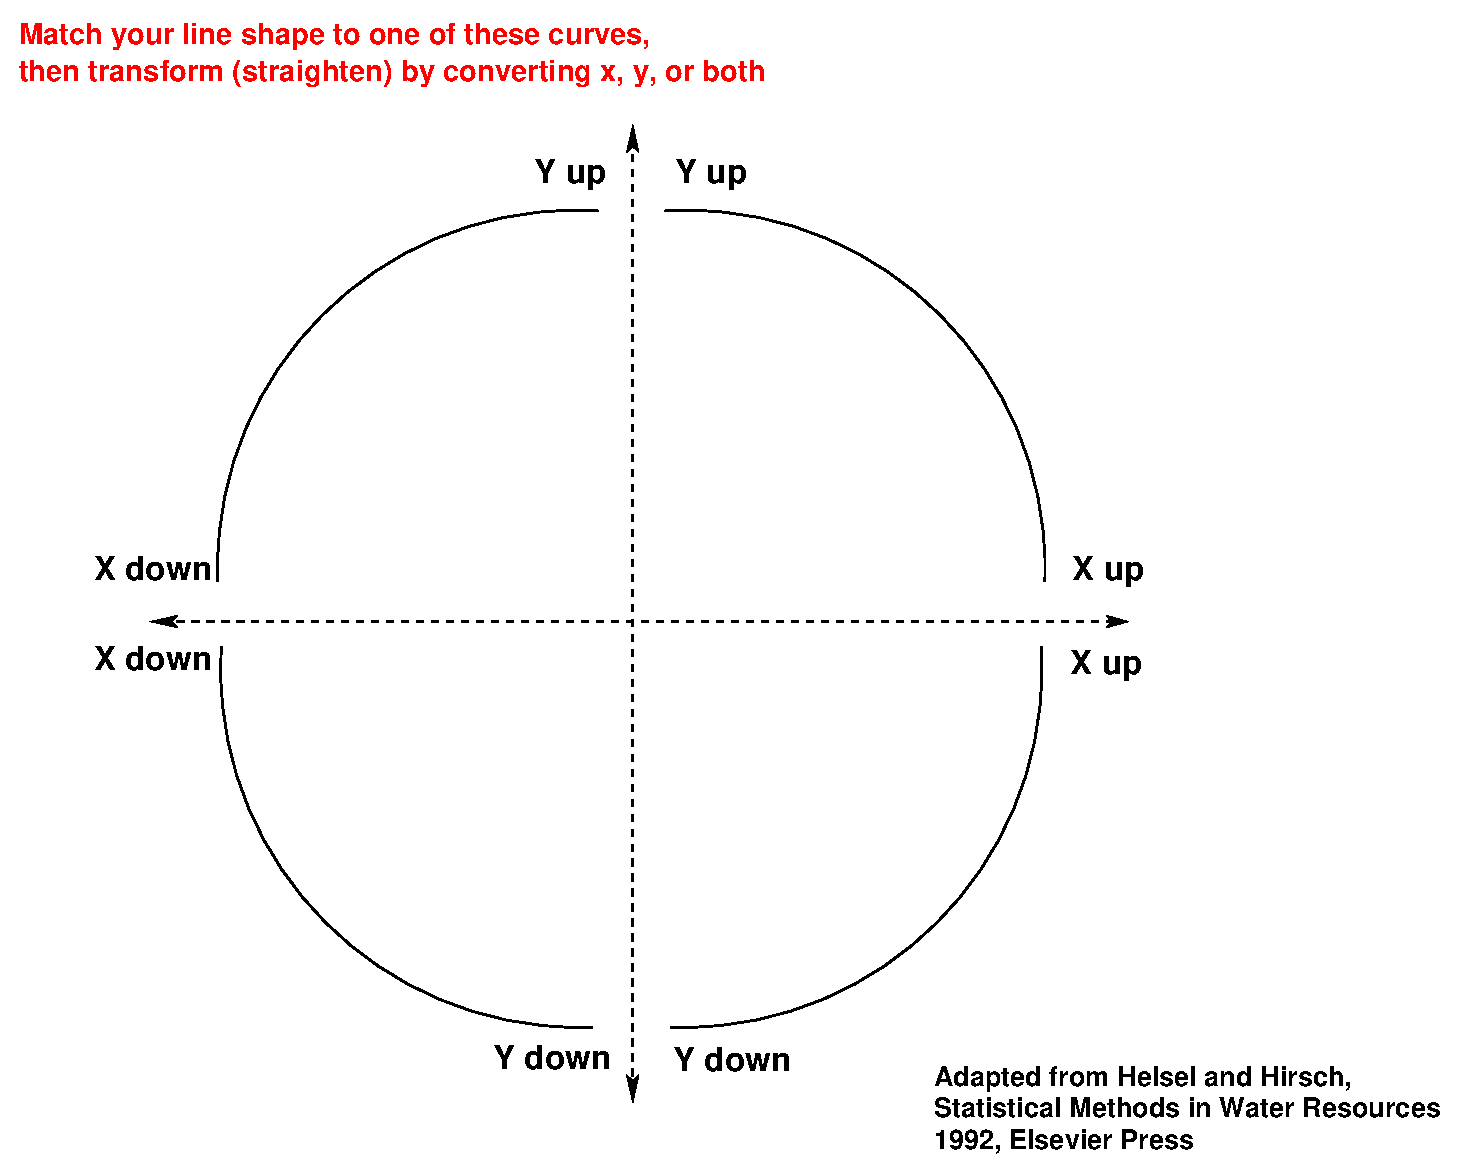
\includegraphics{./part3figures/lop1.eps}}
\end{center}
\end{frame}


\begin{frame}
\frametitle{Regression Transformations}
\framesubtitle{Ladder of Power - {\tt \color{red} R} Syntax}

\begin{center}
\begin{tabular}{|l|l|l|} \hline
Description                     & Transformation        & {\color{red}R Code} \\ \hline
Negative skewness               & Cube                  & {\color{red}Y$\wedge$3}\\
(top of ladder)                 & Square                & {\color{red}Y$\wedge$2}\\
                                & Square root           & {\color{red}Y$\wedge$(1/2)} or {\color{red}sqrt(Y)}\\
                                & Cube root             & {\color{red}Y$\wedge$(1/3)} \\
{\color{blue} center  - start here $\Rightarrow$}  & Log               & {\color{red}log10(Y)}\\
                                & Reciprocal root       & {\color{red}-1/sqrt(Y)}\\
Positive skewness               & Reciprocal            & {\color{red}-1/Y}\\
                                & Reciprocal root       & {\color{red}-1/sqrt(Y)}\\
Positive skewness               & Reciprocal            & {\color{red}-1/Y}\\
(bottom of ladder)              & Reciprocal of square  & {\color{red}-1/(Y$\wedge2$)}\\ \hline
\multicolumn{3}{l}{{\tiny Adapted from Helsel and Hirsch, Statistical Methods in Water Resources}}\\
\end{tabular}
\end{center}


{\footnotesize
Logs other than base 10 can be used\\
Constants can be added to x to avoid dividing by zero ({\color{red} \tt log1p(x)} computes log(1+x))\\
Higher and lower powers can be used\\
}

\end{frame}


\begin{frame}[fragile]
\frametitle{Finding the Best Transformation}
\framesubtitle{Box-Cox Procedure}
\label{BCexample}

\bi
\item The Box-Cox procedure in the {\color{red} \tt MASS} library will
  estimate the ``best'' power (lambda) for transforming Y

\item The procedure defaults to $\pm$2 (Y$^{-2}$ to Y$^2$)

{\scriptsize
\color{red}
\verb%X <- c(1:10)%\\
\verb%Y <- c(0.021,0.671,1.094,1.390,1.602,1.792,1.950,2.085,2.201,2.311)%\\
\verb%### Y is ln(X) plus noise%\\

\vspace{2ex}
\verb%Yfit <- lm(Y~X)%\\

\vspace{2ex}
\verb%library(MASS)%\\
\verb%Yfit.bc <- boxcox(Yfit)%\\
\verb%Yfit.bc$x[which.max(Yfit.bc$y)]%\\

\vspace{1ex}
\color{blue}
\verb%[1] 2%\\

\vspace{2ex}
\color{red}
\verb%##### Best est. for transformation will be Y^2%\\
\verb%YfitBC.trans <- lm(Y^2 ~ X)%\\
}

\ei
\end{frame}


\begin{frame}
\frametitle{Example of Transforming Y to Y$^2$}
\begin{center}
\resizebox{3in}{!}{
\includegraphics{./part3figures/Y2bc.ps}}
\end{center}
\end{frame}

\begin{frame}[fragile]
\frametitle{Advanced Plotting Example}
\framesubtitle{Plotting Linear Models and Residuals With/Without Transformation}

{\scriptsize Plotting example uses data and Box-Cox transformation
  show on page \pageref{BCexample}}

{\tiny
\color{red}
\begin{verbatim}
### Set plotting output to 4x per page
par(mfrow=c(2,2))

### Plot untransformed Y and residuals from Yfit
plot(Y ~ X, main="Y vs X, untransformed",  pch=21, bg="red", cex=1.5)
abline(Yfit, lwd=2, lty=2, col="red")
legend(x="topleft", c(paste("Y =", round(Yfit$coef[2],4),
         "* X + ", round(Yfit$coef[1], 4)),
         paste("Adj.R-squared =", round(summary(Yfit)$adj.r.squared, 4)),
         paste("p-value =", round(summary(Yfit)$coef[8], 4))),
         bty="n", cex=0.7)
plot(Yfit$fitted.values, resid(Yfit), main="Untransformed residuals",
     pch=21, bg="red", cex=1.5,  xlab="Fitted Values", ylab="Residuals")
abline(h=0, lwd=2, lty=2, col="red")

### Plot transformed Y using Box-Cox estimate and YfitBC residuals
plot(Y^2 ~ X, main="Y^2 vs X", pch=21, bg="red", cex=1.5)
abline(YfitBC.trans, lwd=2, lty=2, col="red")
legend(x="topleft", c(paste("Y^2 =", round(YfitBC.trans$coef[2],4),
         "* X ", round(YfitBC.trans$coef[1], 4)),
         paste("Adj.R-squared =", round(summary(YfitBC.trans)$adj.r.squared, 4)),
         paste("p-value =", round(summary(YfitBC.trans)$coef[8], 4))),
         bty="n", cex=0.7)
plot(YfitBC.trans$fitted.values, resid(YfitBC.trans), main="Transformed residuals",
     pch=21, bg="red", cex=1.5, xlab="Fitted Values", ylab="Residuals")
abline(h=0, lwd=2, lty=2, col="red")
\end{verbatim}
}
\end{frame}



\begin{frame}
\frametitle{Example of Transforming to Y to exp(Y)}
\begin{center}
\resizebox{3in}{!}{
\includegraphics{./part3figures/Y2exp.ps}}
\end{center}
\end{frame}

\begin{frame}[fragile]
\frametitle{Examining Transformations Using Density Plots}
\begin{center}
\resizebox{2.75in}{!}{
\includegraphics{./part3figures/advanced2.ps}}
\end{center}

\vspace{-3ex}
{\scriptsize \color{red}
\verb%##### basic plotting code:%\\
\verb%plot(density(alk)); plot(density(log(alk))); plot(density(sqrt(alk)))%\\
}
\end{frame}

\begin{frame}[fragile]
\frametitle{Examining Transformations Using QQ Plots}
\begin{center}
\resizebox{2.5in}{!}{
\includegraphics{./part3figures/advanced3.ps}}
\end{center}
\vspace{-2ex} 

{\scriptsize QQ plots are a simply way to explore distributions; if
  the data are normally distributed, the points will be close to the
  diagonal reference line. Syntax: {\color{red} \tt qqnorm(alk);
    qqline(alk)} \\}
\end{frame}


\begin{frame}
\begin{center}
\resizebox{3in}{!}{
\includegraphics{./part3figures/advanced4.ps}}
\end{center}
\end{frame}

\begin{frame}[fragile]
\frametitle{Multiple Linear Regression}

\bi
\item The equation for multiple regression is a logical expansion of the basic linear model:

\hspace{5ex}$y_{i} = a + b_{1}u_{i} + b_{2}v_{i} + b_{3}w_{i} + \varepsilon_{i}$

\hspace{10ex}$a$ = intercept\\
\hspace{10ex}$b$ = slopes associated with variables $u$, $v$, and $w$\\
\hspace{10ex}$\varepsilon$ = residual for the i$^{th}$ observation

{\color{red} \tt R} syntax: {\color{red} \verb%lm(y ~ u + v + w)%\\}

\item For linear regressions with interaction terms, the model becomes:

\hspace{5ex}$y_{i} = a + b_{1}u_{i} + b_{2}v_{i} + b_{3}u_{i}v_{i} + \varepsilon_{i}$

{\color{red} \tt S} syntax: {\color{red} \verb%lm(y ~ u * v)%\\}

\item Interpreting the output and selecting the best subset of
  variables for the final multiple regression model in not simple!
\ei
\end{frame}



\begin{frame}
\frametitle{Analysis of Variance}

\bi
\item Analysis of variance procedures ($t$ test, ANOVA, MANOVA)
  use ratios of within-group variance to total variance to test for
  significant differences between groups

H$_{o}$: $\overline{x_1} = \overline{x_2} = \ldots \overline{x_n}$ \hspace{3ex} ($n$ = number of groups)

H$_{a}$: $\overline{x_1} \ne \overline{x_2} \ne \ldots \overline{x_n}$ 

\item The decision to accept or reject the null hypothesis carries a
  probability ($p$) of committing a Type I error, which is rejection
  of the null hypothesis when it is actually true.

\item ANOVA tests whether {\em any} of the groups are
significantly different

\item ANOVA is often used in conjunction with a multiple range test to
determine which groups are different from the others.
\ei
\end{frame}


\begin{frame}
\frametitle{ANOVA}
\framesubtitle{Type I and II Errors}

\bi
\item Type I errors become more likely when you repeat ANOVA on
  subgroups of the data (use p-value adjustment)

\item Type II errors usually indicates a small samples size, but can
  also be caused by extremely large samples sizes (use {\color{red}
    \tt sample})

\ei

\vspace{2ex}
\begin{center}
\begin{tabular}{|c|c|c|}\hline
Decision                        & H$_{o}$ is true       & H$_{o}$ is false \\ \hline
Accept H$_{o}$                  & ok                    & Type II error \\
(Fail to Reject H$_{o}$)        & Prob = 1--$\alpha$    & Prob = $\beta$ \\ \hline
Reject H$_{o}$                  & Type I error          & ok\\
                                & Prob = $\alpha$       & Prob = 1--$\beta$\\ \cline{2-3}
                                & {\bf Significance level}      & {\bf Power}\\ \hline
\end{tabular}
\end{center}
\end{frame}



\begin{frame}
\frametitle{ANOVA}
\framesubtitle{Assumptions for Analysis of Variance (ANOVA)}
\bi
\item  ANOVA is based on several important assumptions:
        \bi
        \item The samples were collected randomly 
        \item The measured variables are distributed normally within each group
        \item The variances are homogeneous (homoscedastic) across groups
        $\Rightarrow$ very important assumption!
        \ei

\item Most uses of ANOVA rely heavily on its ability to perform
  despite departures from normality and homogeneity
 
\item Nonparametric versions of ANOVA are easy to use, powerful, and avoid
the issue of normality and homogeneity

\ei
\end{frame}



\begin{frame}[fragile]
\frametitle{ANOVA}
\framesubtitle{Testing Assumption of Normality}

\bi
\item You want to {\em accept} the hypotheses H$_{o}$ that the data
  from each group fits a normal distribution (p-value $>$0.050)

\item The Shapiro-Wilks test of normality is simple in {\color{red} \tt R}:

\vspace{1ex}
{\scriptsize
\color{red}
\verb%data(iris); attach(iris)%\\
\verb%shapiro.test(Sepal.Length[Species=="setosa"])%\\

\vspace{1ex}
\color{blue}
\verb%        Shapiro-Wilk normality test%\\
\verb%data:  Sepal.Length[Species == "setosa"]%\\
\verb%W = 0.9777, p-value = 0.4595%

\verb%##### edited output for remaining iris species%\\
\verb%data:  Sepal.Length[Species == "versicolor"]%\\
\verb%W = 0.9778, p-value = 0.4647%

\verb%data:  Sepal.Length[Species == "virginica"]%\\
\verb%W = 0.9712, p-value = 0.2583%\\
}

\item Alternatively, you could use {\color{red} \tt qqnorm} to examine the data graphically
\ei
\end{frame}


\begin{frame}[fragile]
\label{variancetests}
\frametitle{ANOVA}
\framesubtitle{Testing Assumption of Variance Homogeneity}

\bi
\item You want to {\em accept} the H$_{o}$ that variances are homogeneous

\item Use Bartlett's test if the data are normally distributed or
  Fligner's test if you don't want to make that assumption

{\scriptsize \color{red}
\verb%bartlett.test(Sepal.Length, Species)%\\
\color{blue}
\verb%        Bartlett test for homogeneity of variances%\\
\verb%data:  Sepal.Length and Species%\\
\verb%Bartlett's K-squared = 16.0057, df = 2, p-value = 0.0003345%

\vspace{1ex}
\color{red}
\verb%fligner.test(Sepal.Length, Species)%\\
\color{blue}
\verb%        Fligner-Killeen test for homogeneity of variances%\\
\verb%data:  Sepal.Length and Species%\\
\verb%Fligner-Killeen:med chi-squared = 11.618, df = 2, p-value = 0.003000%\\
}

\item The sepal length data fail the assumption of
  homoscedasticity!\\ 

\vspace{1ex}
{\scriptsize {\em Optional exercise:} Modify the syntax to show that a
log transformation of the sepal length data corrects the
heteroscedasticity problem\\}

\item You could also use {\color{red} \tt boxplots} to examine the data
  graphically \ei
\end{frame}


\begin{frame}[fragile]
\frametitle{ANOVA Using {\color{red} \tt R}}

\bi
\item The simplest {\color{red} \tt R} syntax for ANOVA uses {\color{red}
  \tt aov}

{\scriptsize \color{red}
\verb%##### Untransformed sepal lengths %\\
\verb%data(iris); attach(iris)%\\
\verb%aov.SL <- aov(Sepal.Length ~ Species)%\\
\verb%summary(aov.SL)%\\

\vspace{1ex}
\color{blue}
\verb%             Df Sum Sq Mean Sq F value Pr(>F)    %\\
\verb%Species       2  63.21  31.606   119.3 <2e-16 ***%\\
\verb%Residuals   147  38.96   0.265                   %\\
\verb%---%\\
\verb%Signif. codes:  0 ‘***’ 0.001 ‘**’ 0.01 ‘*’ 0.05 ‘.’ 0.1 ‘ ’ 1 %\\

\vspace{2ex}
\color{red}
\verb%##### Log-transformed sepal lengths %\\
\verb%aov.logSL <- aov(log(Sepal.Length) ~ Species)%\\
\verb%summary(aov.logSL)%\\

\vspace{1ex}
\color{blue}
\verb%             Df Sum Sq Mean Sq F value Pr(>F)    %\\
\verb%Species       2  1.892  0.9459   128.9 <2e-16 ***%\\
\verb%Residuals   147  1.079  0.0073                   %\\
}

\item Both tests indicate that there are significant differences between the
sepal lengths for the different iris species
\ei

\end{frame}

\begin{frame}[fragile]
\frametitle{ANOVA Using {\color{red} \tt R}}
\framesubtitle{Adding Post-Hoc Tests}

\bi
\item The ANOVA doesn't tell us which species are different, so we use
  a {\em post-hoc} test

\item {\em Which} post-hoc test to use is beyond the scope of this
  class $\ldots$ there are many choices

\item Most {\color{red} \tt R} textbooks use {\color{red} \tt
  pairwise.t.test}, which does 2-group ANOVAs, correcting the p-value
  for repeated testing (Type I errors)

\item The post-hoc test should use log-transformed data (see
  page \pageref{variancetests})

{\scriptsize \color{red}
\verb%pairwise.t.test(log10(Sepal.Length), Species)%\\

\color{blue}
\vspace{1ex}
\verb%	Pairwise comparisons using t tests with pooled SD %\\

\verb%data:  log10(Sepal.Length) and Species %\\

\verb%           setosa  versicolor%\\
\verb%versicolor < 2e-16 -         %\\
\verb%virginica  < 2e-16 1.3e-08   %\\

\verb%P value adjustment method: holm %\\
}
\ei
\end{frame}

\begin{frame}[fragile]
\frametitle{Nonparametric Alternatives to ANOVA}

\bi
\item The Kruskal-Wallis rank sum test ({\color{red} \tt
  kruskal.test}), paired with the Wilcoxon rank sum test ({\color{red}
  \tt pairwise.wilcox.test}) will provide a nonparametric alternative
  to ANOVA

\item For {\em untransformed} heteroscedastic data, the nonparametric
  results are usually far more useful than anything based on variance

{\scriptsize \color{red}
\verb%kruskal.test(Sepal.Length ~ Species)%\\

\vspace{1ex}
\color{blue}
\verb%	Kruskal-Wallis rank sum test%\\

\verb%data:  Sepal.Length by Species %\\
\verb%Kruskal-Wallis chi-squared = 96.9374, df = 2, p-value < 2.2e-16%\\

\vspace{2ex}
\color{red}
\verb%pairwise.wilcox.test(Sepal.Length, Species)%\\

\color{blue}
\verb%	Pairwise comparisons using Wilcoxon rank sum test %\\

\verb%data:  Sepal.Length and Species %\\

\verb%           setosa  versicolor%\\
\verb%versicolor 1.7e-13 -         %\\
\verb%virginica  < 2e-16 5.9e-07   %\\

\verb%P value adjustment method: holm %\\
}

\ei

\end{frame}

\begin{frame}
\frametitle{Supplemental References}
\bi
\item Crawley, Michael J.  2013.  The R Book.  John Wiley \& Sons. ISBN 978-0-470-97392-9.

\item Faraway, Julian J.  2014.  Linear Models with R, 2nd Edition.
  CRC Press. ISBN 978-1-439-88733-2.

\item Lander, Jared P.  2014.  R for Everyone, Advanced Analytics and Graphics.  Addison Wesley Data \& Analytics Series,  ISBN 978-0-321-88803-7.

\item Teetor, Paul. 2011.  The R Cookbook.  O'Reilly Publishers. ISBN
  978-0-596-880915-7

\ei

\end{frame}
\end{document}
\end

